\documentclass[11pt,letterpaper,oneside,pagesize]{scrartcl}
\KOMAoptions{BCOR=0mm,DIV=13}

\usepackage[T1]{fontenc}
\usepackage[utf8]{inputenc}
\usepackage{microtype}
\usepackage[lucidasmallscale, nofontinfo]{lucimatx}
%\usepackage{mathpazo}

\usepackage[square,numbers]{natbib}
\usepackage{bibentry}
\usepackage{wrapfig}


\usepackage{booktabs}
\usepackage{units}
\usepackage{pdfpages}
\usepackage{paralist}
\usepackage{subfigure}
\usepackage[version=3]{mhchem}
\mhchemoptions{arrows=pgf}
\usepackage{tikz}

\usepackage{fancybox}
\usepackage{marginnote}
\renewcommand*{\marginfont}{\small\itshape}

\usepackage{xspace}

%\usepackage[small,compact]{titlesec}

% for figures
\usepackage[margin=10pt,font=small]{caption}
\usepackage{subcaption}
\usepackage{graphicx}
\usepackage[usenames, dvipsnames]{xcolor}


% Assignment box environment

\usepackage{fancybox}
\usepackage{fancyvrb}

\newcounter{assign_num}
\setcounter{assign_num}{1}
\newenvironment{assignment}%
{\begin{Sbox}\begin{minipage}{6in}%
\textbf{Assignment \arabic{assign_num}\stepcounter{assign_num}}:}% 
{\end{minipage}\end{Sbox}\shadowbox{\TheSbox}}


% Comment box environment

\newenvironment{commentbox}%
{\setlength{\fboxsep}{15pt}%
\begin{Sbox}%
\begin{minipage}{6in}%
\sffamily \vspace*{1ex}%
\textbf{\large Comments}\vspace*{0.5ex}\color{red}\\}% 
{\vspace*{0.5ex}%
\end{minipage}\end{Sbox}\ovalbox{\TheSbox}}

\newenvironment{comment}[1]{\vspace*{2ex}\sffamily \color{red} #1}{\vspace*{2ex}}



%% Fancy syntax coloring via pygments
\usepackage{minted}
\usemintedstyle{bw}

\definecolor{bg}{rgb}{0.96,0.96,0.96}

\newenvironment{Rcode}
{\VerbatimEnvironment
 \begin{minted}[xleftmargin=1em, baselinestretch=0.88]{r}}%
{\end{minted}}


\newenvironment{Pcode}
{\VerbatimEnvironment
 \begin{minted}[xleftmargin=1em,baselinestretch=0.88]{python}}%
{\end{minted}}

\newenvironment{Code}[1]
{\VerbatimEnvironment
 \begin{minted}[framesep=0.5em,xleftmargin=1em]{#1}}%
{\end{minted}}


\newenvironment{PageCode}[1]
{\VerbatimEnvironment
 \begin{minted}[frame=single, framerule=1.5pt,framesep=0.5em,xleftmargin=1em]{#1}}%
{\end{minted}}

% \DefineShortVerb{\|} 
% \everymath{\UndefineShortVerb{\|}\vert}


\newcommand{\Species}[1]{{\rmfamily \itshape #1}}

% Math related macros
\newcommand{\Real}{\ensuremath{\mathbb{R}}}
\newcommand{\RealN}{\ensuremath{\mathbb{R}^n}}
\newcommand{\RealP}{\ensuremath{\mathbb{R}^p}}
\newcommand{\Mtx}[1]{\ensuremath{\mathbf{#1}}}
\newcommand{\Inv}[1]{\ensuremath{#1^{-1}}}
\newcommand{\InvMtx}[1]{\ensuremath{\mathbf{#1}^{-1}}}
\newcommand{\Red}[1]{\textcolor{red}{#1}}
\newcommand{\PsInv}[1]{\ensuremath{\mathbf{#1}^{+}}}




% Hyperref should be the last package
\usepackage{hyperref}
\hypersetup{
colorlinks=true
}


%% these two should always be the last packages loaded
\usepackage[colorlinks=true,citecolor=blue,linkcolor=black]{hyperref}
\usepackage[capitalize]{cleveref} % should always be loaded after hyperref



\title{BIO723: Scientific Computing for Biologists}
\author{Paul M. Magwene\\Fall 2012}



\begin{document}
\maketitle

In this lecture I focus on developing a few simple analytical models. The exposition and models described here are drawn from:

\nobibliography{signaling-refs}
\bibliographystyle{plainurl}
\begin{enumerate}
    \item \bibentry{Alon2007}
    \item \bibentry{Shen-Orr2002}
    \item \bibentry{Alon2007book}
\end{enumerate}

\section{Reaction Equations}

The chemical kinetics ``Law of Mass Action'' states that the rate of a reaction is proportional to the concentrations of the reactants. For example, if the reaction is given by:
%
\begin{center}
    $A$ \ce{->[k]} $B$
\end{center}
%
then
%
\[
\frac{d[A]}{dt} = -k[A] \qquad  \mbox{and} \qquad \frac{d[B]}{dt} =  k[A]
\]
%
where $t$ is time and $k$ is a constant reaction rate, and where the brackets indicate the concentrations of the reactants.

Similarly for bimolecular reactions:
\begin{center}
$A + B$ \ce{->[k]} $C$
\end{center}
the reaction rates are given by:
\begin{eqnarray*}
\frac{d[A]}{dt} & = & -k[A][B] \\
\frac{d[B]}{dt} & = & -k[A][B] \\
\frac{d[C]}{dt} & = & k[A][B] \\
\end{eqnarray*}
This can be extended to an arbitrary number of reactants.

\subsection{Reversible Reactions}

Most chemical and biological reactions are reversible:
\begin{center}
    $A$ \ce{<=>[k_1][k_{-1}]} $B$
\end{center}
%
At equilibrium none of the concentrations are changing ($k_1[A] = k_{-1}[B]$)
and therefore
\[
[A][B] = k_{-1}/k_1 = K_{\mathrm{eq}}\qquad \mbox{(the equilibrium constant)}
\]
%
For a reversible bimolecular reaction:
\begin{center}
    $A + B$ \ce{<=>[k_1][k_{-1}]} $C$
\end{center}
and at equilibrium $k_1[A][B] = k_{-1}[C]$ so that $[A][B]/[C] = k_{-1}/k_1 = K_{eq}$. For bimolecular reactions $k_1$ is often refered to as the association constant ($k_{\mathrm{on}}$) while $k_{-1}$ is the dissociation constant ($k_{\mathrm{off}}$).

\section{Enzyme-catalyzed reactions}

Enzymes accelerate the rates of reactions, but do not affect their equilibrium. In other words, enzymes increase the values of the $k$'s but do not affect $K_{eq}$.

The general scheme for an enzymatic reaction is:

\begin{center}
    \ce{S + E <=>[k_1][k_{-1}] ES <=>[k_2][k_{-2}] E + P}
\end{center}
%
This describes an enzyme, $E$ binding it's substrate $S$ to form an enzyme-substrate complex $ES$. At the end of the reaction the substrate $S$ is converted into product $P$ and the enzyme is unaltered. Most if not all enzymatic reactions are reversible.

Enzymatic reactions do not follow mass action kinetics because there is usually a limited amount of enzyme present. If we assume that the rate at which $E + P$ forms is very fast compared to the rate at which $ES$ dissociates back to $E + S$, then after a very brief period, a steady-state will be stablished in which $[ES]$ is essentially constant over time. We further assume the $P$ does not accumulate (e.g. it is very rapidly removed by another reaction), so the overall scheme becomes:
%
\begin{center}
    \ce{S + E <=>[k_1][k_{-1}] ES ->[k_2] E + P}
\end{center}
%
Under those assumptions, simple enzymatic reactions are well approximated by the Michaelis-Menten equation, usually written as:
\[
v = \frac{V_{\max}[S]}{K_m + [S]}
\]
where $v = k_2[ES]$, $V_{\max} = k_2[E_t]$ where $[E_t] = [E] + [ES]$ and $K_m = (k_2+k_{-1})/k_1$.

A graph showing the rate of reaction, $v$, as a function of substrate concentration $[S]$ has a hyperbolic shape as shown in \cref{fig:michaelis}

\begin{figure}[lh]
\centering
 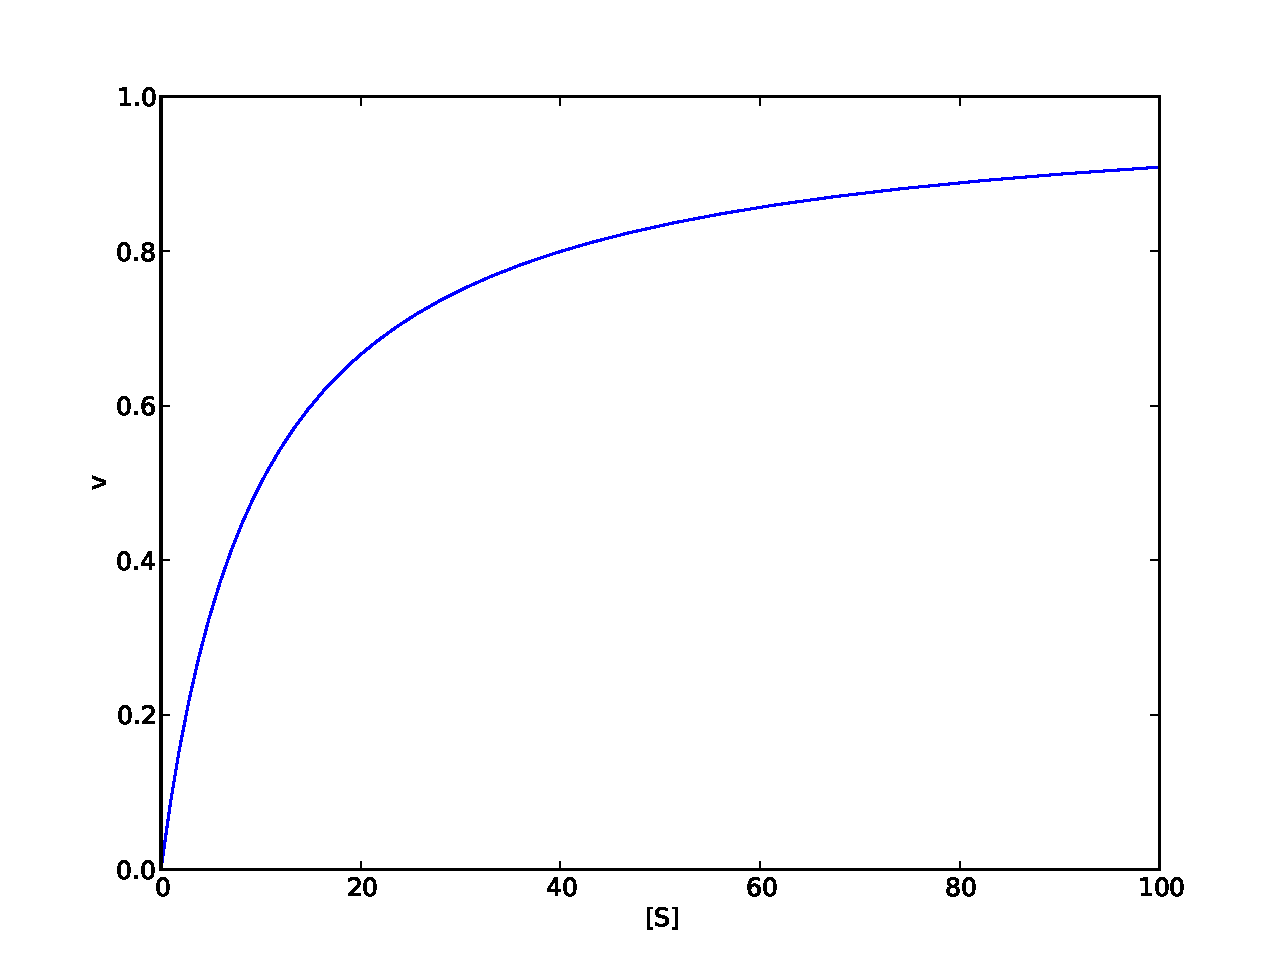
\includegraphics[width=3in]{michaelis-curve.pdf}
\caption{A curve described by the Michaelis-Menten equation with $V_{\max}=1$ and $K_m = 10$.}
\label{fig:michaelis}
\end{figure}



\section{Hill Equation}

Biochemical reactions that are more complex then the simple enzymatic reactions that the Michaelis-Menten equation describes are often described by the Hill Equation.  The Hill equation was originally derived in the context of cooperative enzymatic reactions where an enzyme binds several substrate molecules at the same time and the binding of each subsequent substrate molecules enhances the affinity of the enzyme for the substrate. This sort of cooperative reaction is described by the formula:
%
\[
v = \frac{V_{\max}[S]^n}{K_d + [S]^n}
\]
%
where $V_{\max}$ is the maximum velocity of the reaction, $[S]$ is the concentration of the substrate, and $K_d$ is the dissociation constant. The Michaelis-Menten equation can be viewed as a special case of the Hill equation with $n=1$.

The Hill equation, written in this form, describes a sigmoid relationship between the substrate concentration and the velocity of the reaction. The larger the value of $n$ the more `step-like' the relationship as illustrated in the \cref{fig:hillcurves}. The Hill equation is also used to describe non-enzymatic reactions. For example, consider a transcription factor, $X$, that positively regulates the transcription of gene $Y$.  We describe the rate of production of $Y$ as $f(X)$ where:

\[
f(X) = \frac{\beta X^n}{K^n + X^n}
\]
where $K$ is the `activation coefficient' and is related to the affinity between X and it's binding sites. $\beta$ is the maximum expression level of the promoter, and again $n$ governs the steepness of the function.

\begin{figure}[lh]
\centering
 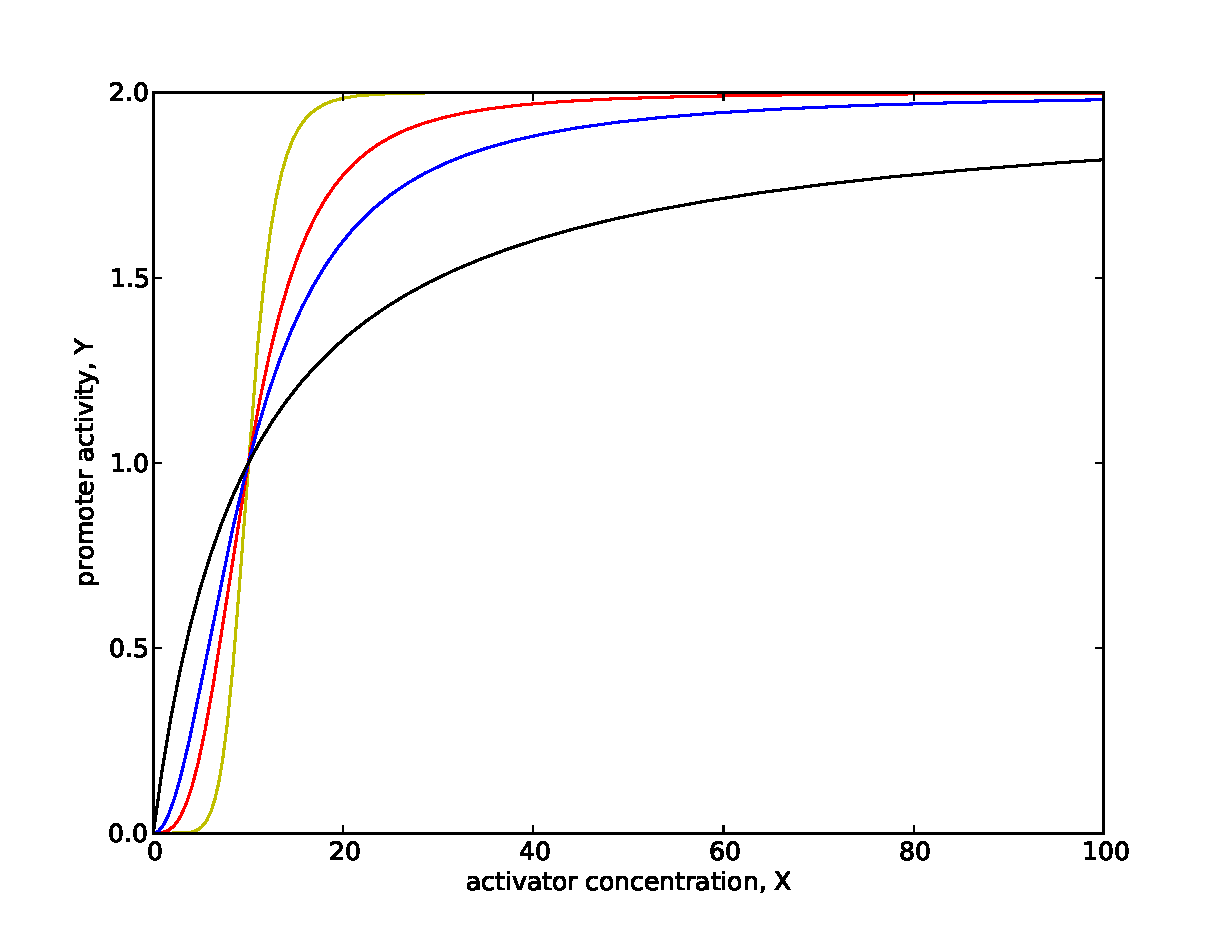
\includegraphics[width=3in]{hillcurves.pdf}
\caption{Hill functions with varying degrees of Hill coefficients describing transcriptional activation -- $n=1$ (black), $n=2$ (blue), $n=3$ (red), $n=8$ (yellow).}
\label{fig:hillcurves}
\end{figure}



If rather than activating Y's transcription, X is a transcriptional repressor we can write:
%
\[
f(X) = \frac{\beta}{1 + (X/K)^n}
\]
%
which yields curves like those shown in \cref{fig:hillrepr}.  Remember that both of these equation describe the production of Y as a function of the levels of X, not the temporal dynamics of Y which we'll look at after developing a few more ideas.

\begin{figure}[lh]
\centering
 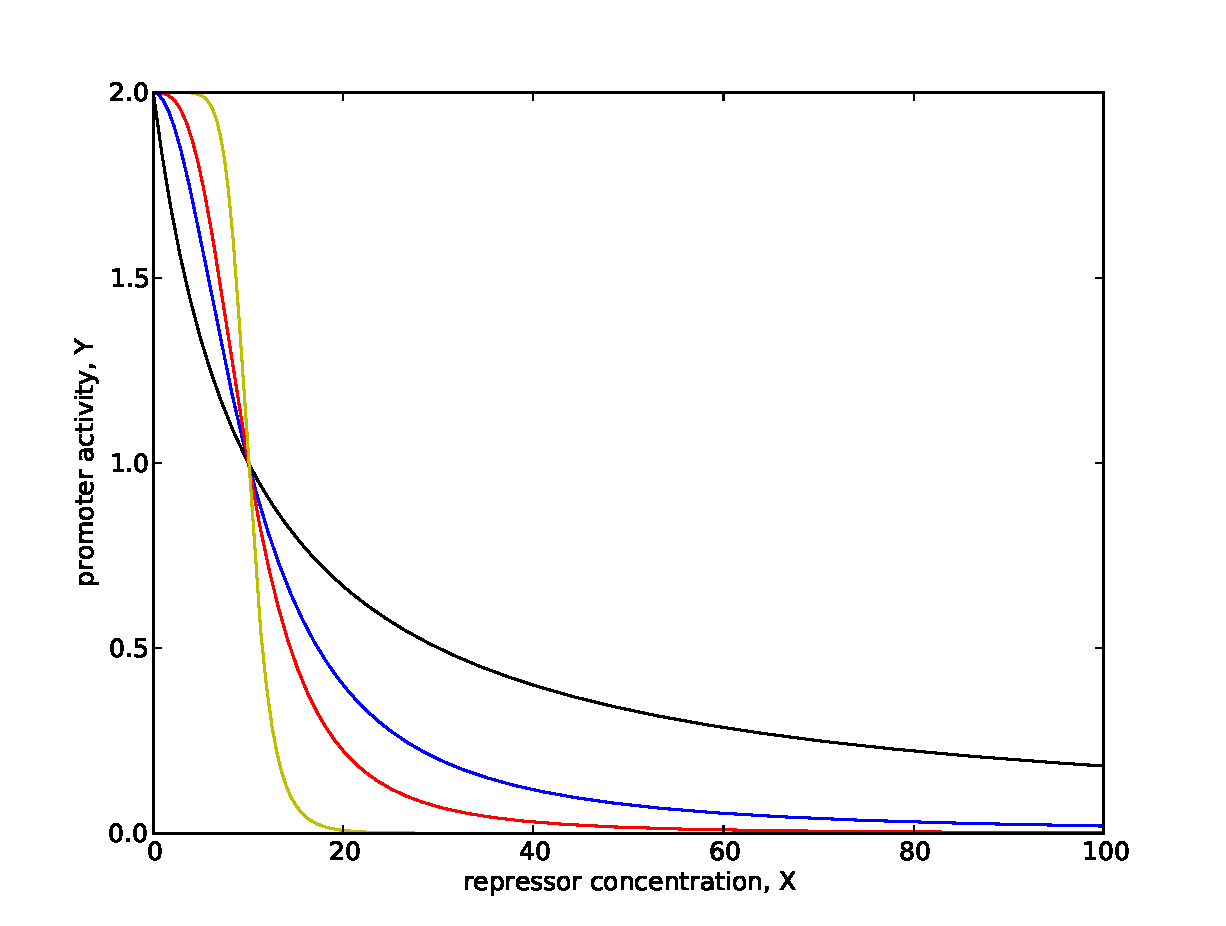
\includegraphics[width=3in]{hillrepr.pdf}
\caption{Hill functions with varying degrees of Hill coefficients describing transcriptional repression -- $n=1$ (black), $n=2$ (blue), $n=3$ (red), $n=8$ (yellow).}
\label{fig:hillrepr}
\end{figure}

% \section{Sensitivity}

% The sensitivity of a signaling system can be defined as the steady-state fractional change in the level of response, $T$, divided by the fractional change in the level of the signal, $S$, for very small changes in $S$:
% \[
% R_{S}^T = \lim_{\Delta S \rightarrow 0} \left(\left(\frac{\Delta T}{T}\right)/\left(\frac{\Delta S}{S}\right)\right) = \frac{d\ln T}{d\ln S}
% \]

% This is essentially equal to the \% change in the level of the response caused by a 1\% change in signal \citep{Kholodenko1997}. $R$ is also known as the response coefficient. If the response coefficient is greater than 1 there is relative amplification of the signal ('sensitivity amplification').

% \begin{figure}[lht]
% \centering
%  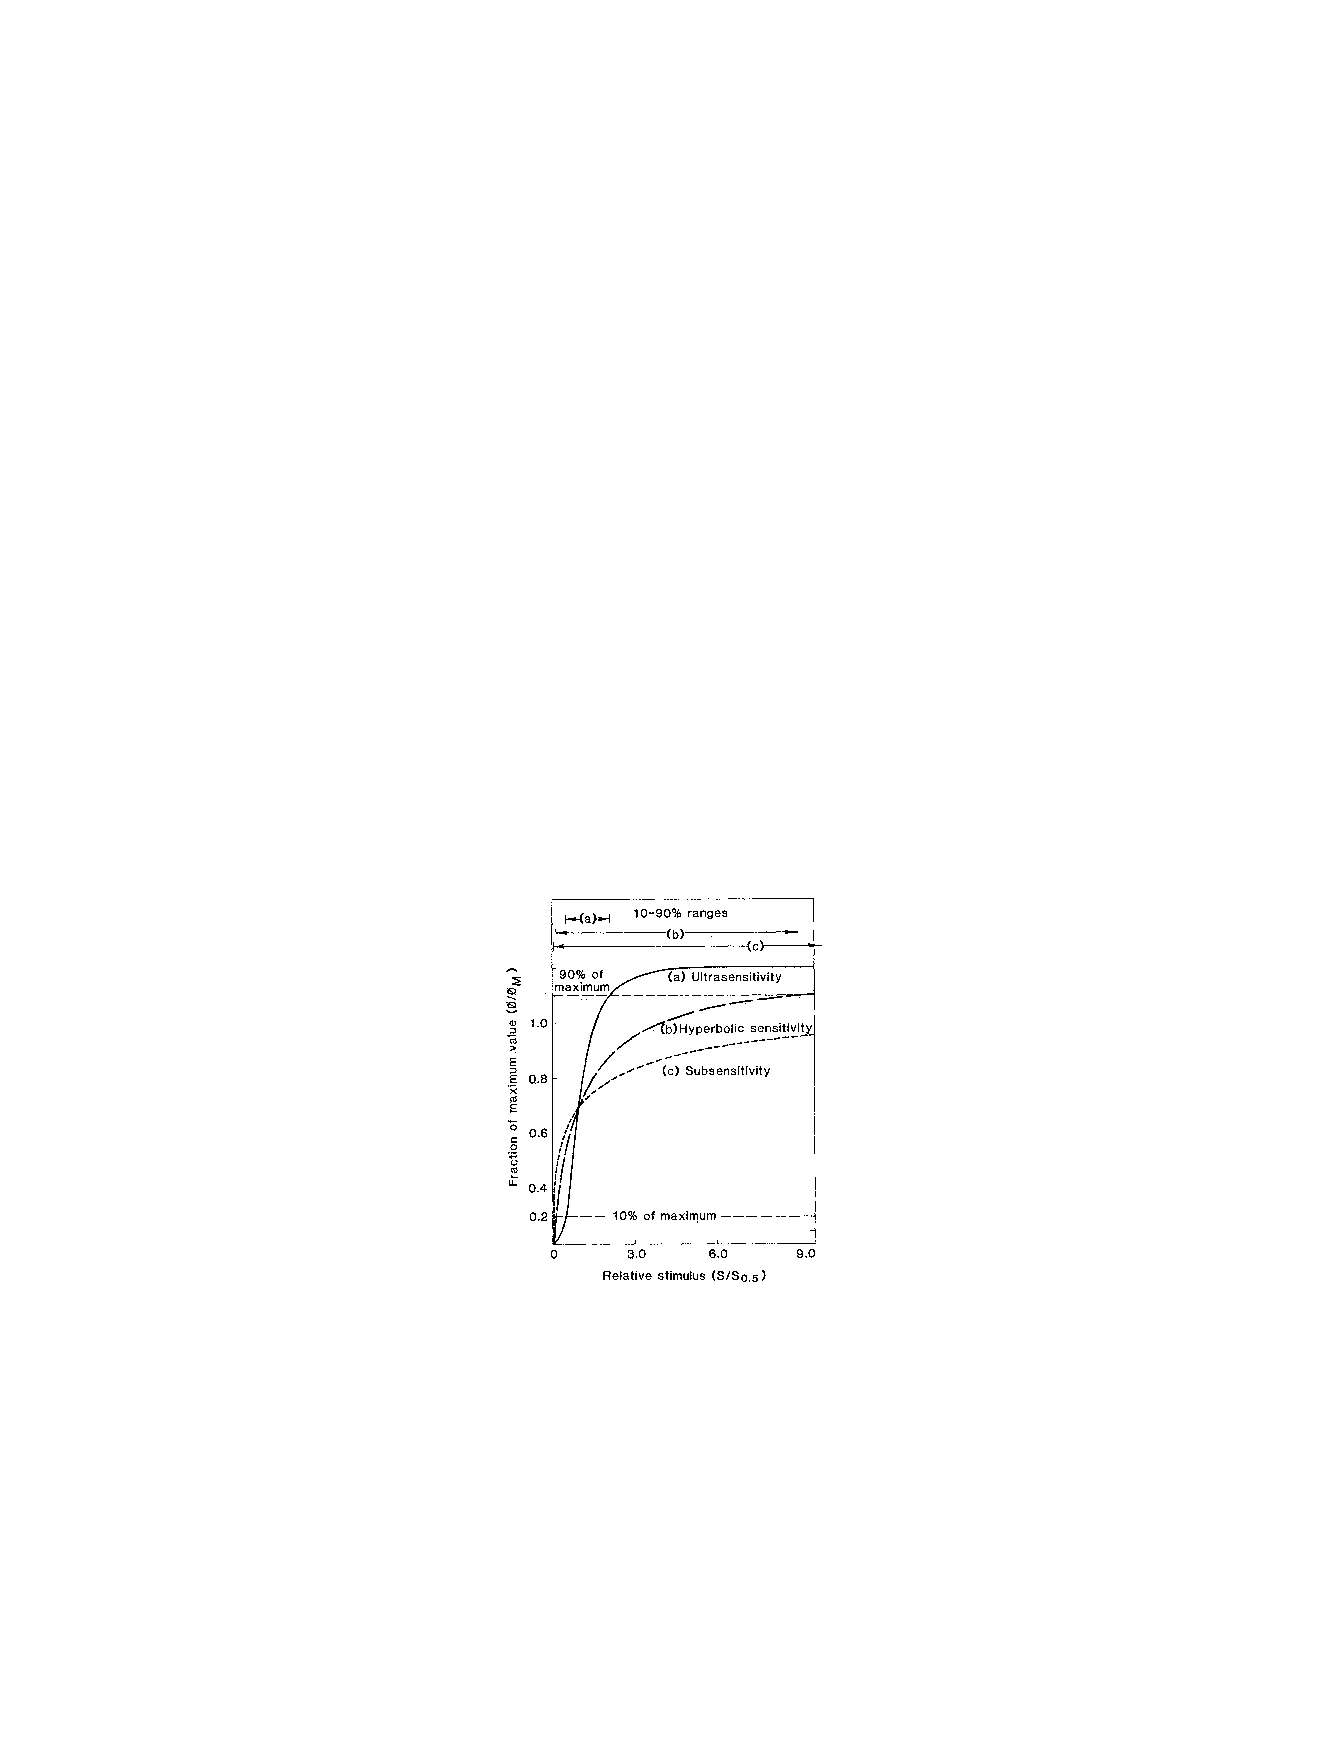
\includegraphics[width=2in]{ultrasensitivity.pdf}
%  \caption{Curves contrasting reactions with hyperbolic (Michaelis), ultrasensitive, and subsensitivity. From \citet{Koshland1982}}
% \label{fig:ultrasensitive}
% \end{figure}

% Biochemists often use the hyperbolic dynamics of Michaelis-Menten type reactions as a benchmark.  Such systems are said to exhibit `hyperbolic sensitivity.' Systems that are more sensitive to stimulus than a Michaelis-Meten system are called `ultrasensitive' while those that are less are called `subsensitive' (Koshland et al. 1982). Systems described by the Hill equation with $n > 1$ are ultrasensitive.  Whether an ultrasensitive system also shows sensitivity amplification depends on the range over which the stimulus-response ratio is observed.


% \section{MAP Kinase Cascades}

% \begin{wrapfigure}{r}{0.23\textwidth}
% \centering
%  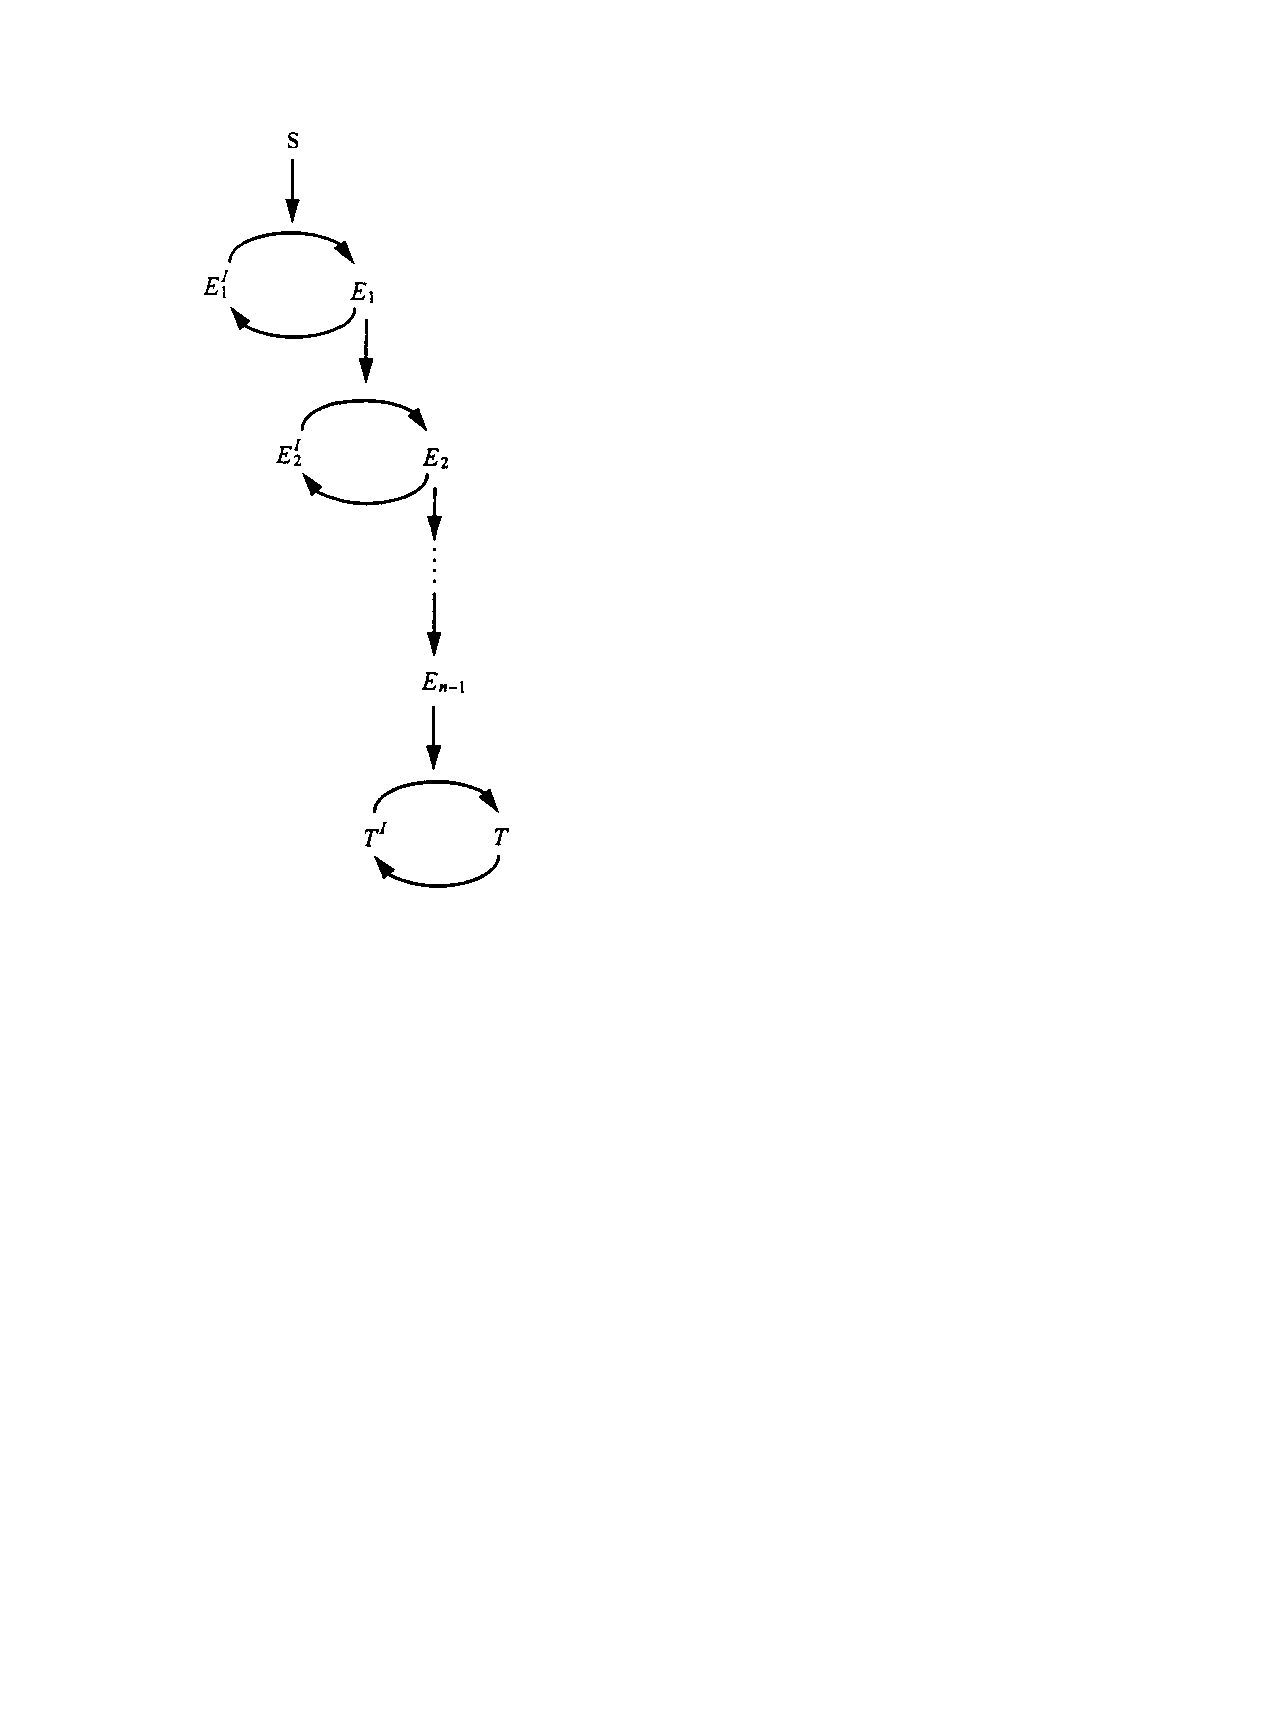
\includegraphics[width=0.2\textwidth]{kholodenko-linear-cascade.pdf}
%  \caption{Figure of a linear cascade from \citet{Kholodenko1997}}
% \label{fig:linearcascade}
% \end{wrapfigure}

% MAP Kinase cascades involve a linear series of phosphorylation reactions. The simplest model is to treat this as a simple linear cascade as in Fig.~\ref{fig:linearcascade}. By simple application of the chain rule (remember your first year calculus course!) one can show that the overall sensitivity of such a cascade is equal to the product of the local sensitivies at each level of the cascade (Kholodenko et al. 1997)

% \[
% R_{S}^T = r_{S}^1 \times r_{1}^2 \times \cdots \times r_{n-1}^T
% \]

% Ferrell (1996) further expands on this idea in a discussion of how MAP kinase cascades can generate sigmoidal, ultransesitive, switch like responses. He writes:

% \begin{quote}
% The answer can be summed up as follows: (1) One level in a cascade passes on any ultrasensitivity to the level below. (2) When two successive levels each exhibit ultransensitivity, equivalent to Hill coefficients of `n' and `m', then their combined response is ultrasensitive with a Hill coefficient that, under certain circumstances, approaches $n \cdot m$. (3) Under other circumstances, the combined response is less than multiplicative.
% \end{quote}

% Our general conclusion from the above is that MAP Kinase cascades will exhibit switch like behavior in response to stimuls if at least a couple levels of the cascade are themselves ultransensitive.  What evidence is there for that?  Let's take a look at a slightly more sophisticated model for what MAP Kinase cascades actually look like (Fig.~\ref{fig:mapk}).

% \begin{figure}[lh]
% \centering
%  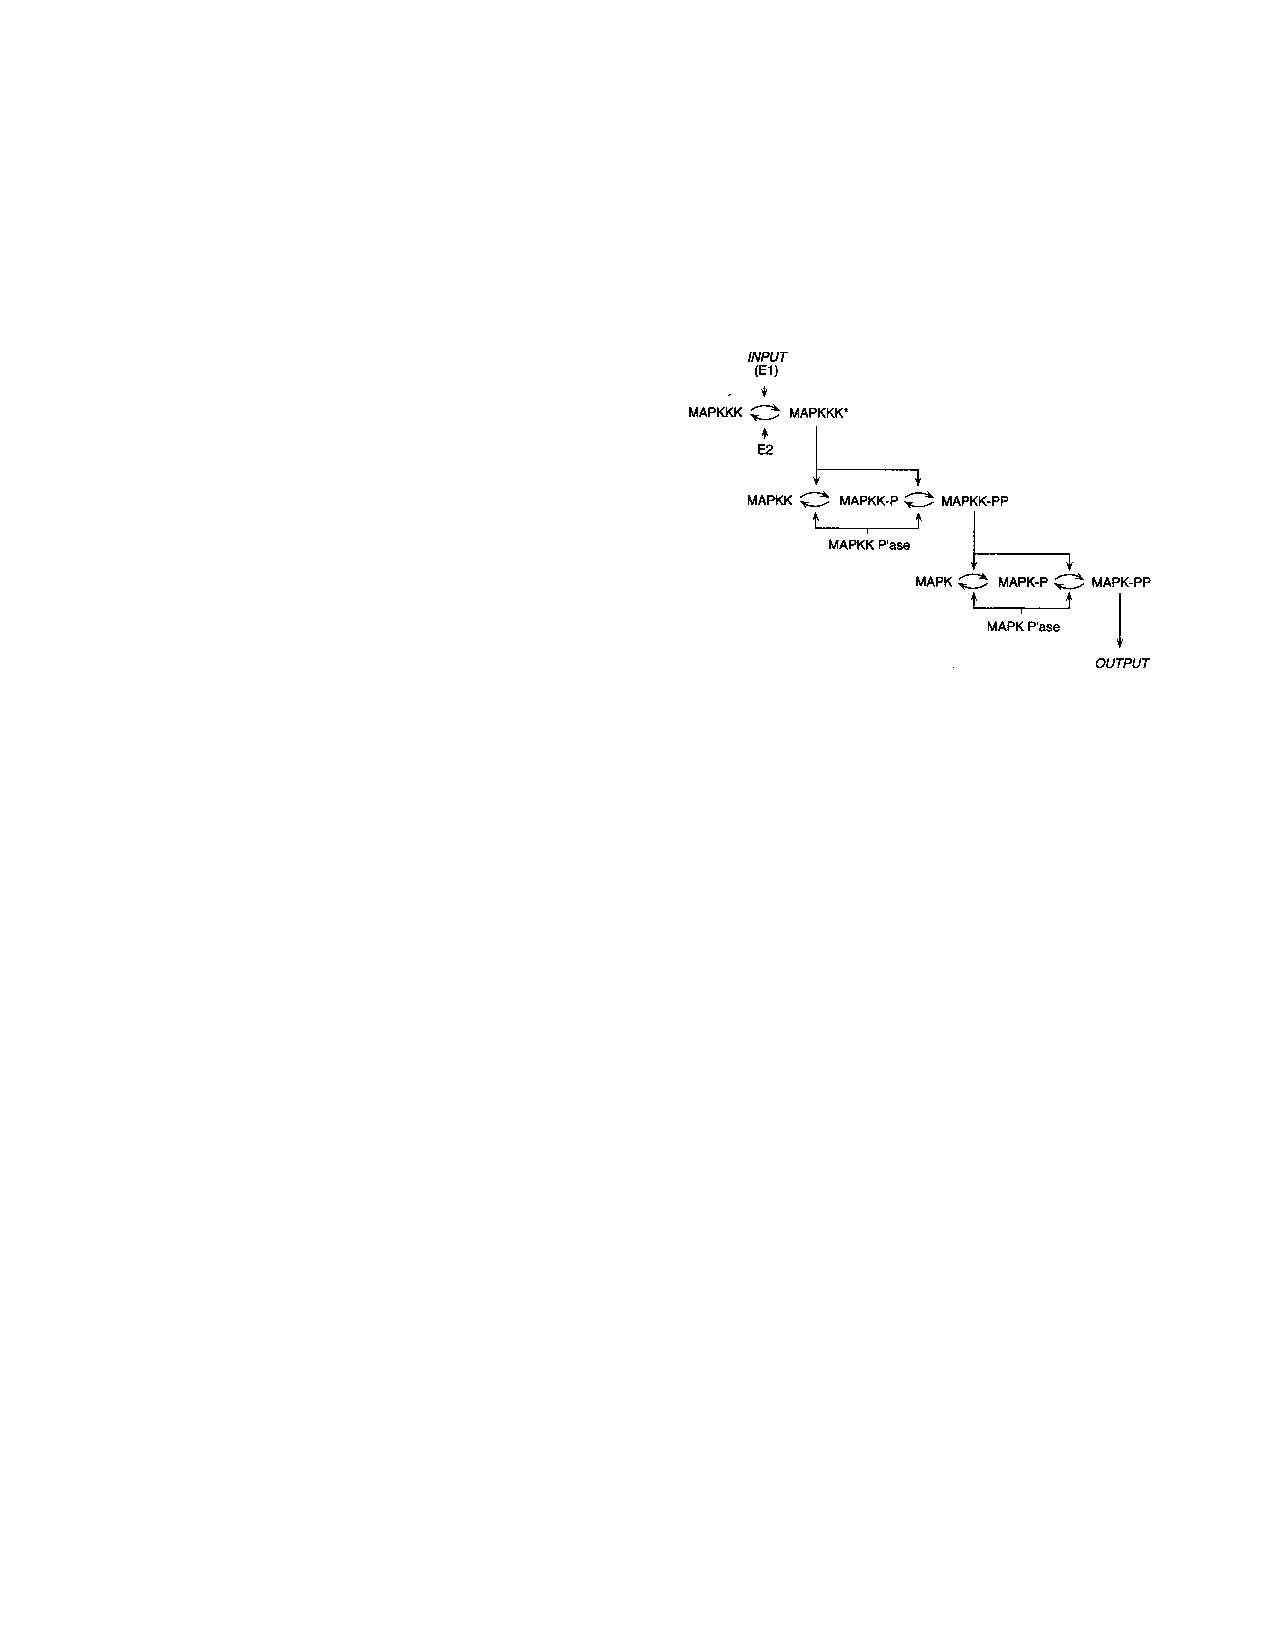
\includegraphics[width=3in]{mapk.pdf}
%  \caption{A schematic of a MAP Kinase cascade from \citet{Huang1996}}
% \label{fig:mapk}
% \end{figure}


% As shown in Fig.~\ref{fig:mapk}, the intermediate kinases in MAP Kinase cascades typically require phosphorylation of \emph{two} residues to become catalytically active.  This requirement for two-step phosphorylation leads to ultransensitivity at the respective individual levels of the cascade (see \citet{Ferrell1996} for a nice graphical derivation of this result).

% A third factor that is thought to increase the switch like behavior of MAP Kinase cascades is positive feedback. For example, Ferrell and Machleder suggest that in \latin{Xenopus} oocytes activated MAPK enhances the phosphorylation of the MAPKK.

\section{Simplifying Models using Logic Approximations}

To simplify analysis it's often convenient to approximate step-like sigmoidal functions like those produced by the Hill equation with functions using logic approximations. We'll assume that a gene, Y, is either on or off -- i.e. $f(X) = 0$ or $f(X) = \beta$. To do this we can rewrite the formula for Y as:

\[
f(X) = \beta\ \Theta(X > K)
\]
where the function $\Theta$ is zero if the statement inside the parentheses is false or one if the statement is true.

When X is a repressor we can write:
\[
f(X) = \beta\ \Theta(X < K)
\]

\subsection{Multi-dimensional Input Functions}

What if a gene needs two or more activator proteins to be transcribed?  We can describe the amount of Z transcribed as a function of active forms of X and Y with a function like:
\[
f(X,Y) = \beta\ \Theta(X > K_x) \Theta(Y > K_y)
\]
The above equation describes `AND' logic (i.e. \emph{both} X and Y have to be above their threshold levels, $K_x$ and $K_y$, for Z to be transcribed). In a similar manner we can define `OR' logic:
\[
f(X,Y) = \beta\ \Theta(X > K_x \mbox{ or } Y > K_y)
\]
A SUM function would be defined like this:
\[
f(X,Y) = \beta_x X + \beta_y Y
\]


\subsection{Dynamics of the Logic Approximation}

Again, let's assume X is a transcriptional activator of Y. For the moment let's assume there is a constant concentration of X (above the threshold $K_y$) so that the rate of production of Y is given by $f(X) = \beta$. Y is lost due to degradation and dilution at a rate, $\alpha$, proportional to the amount of Y. A differential equation to describe the change of Y over time is:
\[
\frac{dY}{dt} = \beta - \alpha Y
\]
At steady state $dY/dt = 0$, which means that the rate of production and the rate of degradation are perfectly balanced ($\beta = \alpha Y$) and we can calculate the steady state value, $Y_{st}$ as:
\[
Y_{st} = \frac{\beta}{\alpha}
\]

Assume Y has come to it's steady state. What happens if we take away the activating signal, X? (i.e. $\beta$ suddenly becomes zero). In that case:
\[
\frac{dY}{dt} = -\alpha Y
\]
and solving for Y as a function of time, $t$, we get:
\[
Y(t) = Y_{st}e^{-\alpha t}
\]
In a similar manner we can consider the case where Y is initially zero. If we solve the differential equation $dY/dt = \beta - \alpha Y$ we find:
\[
Y(t) = Y_{st}(1 - e^{-\alpha t})
\]

\begin{figure}[lht]
\centering
 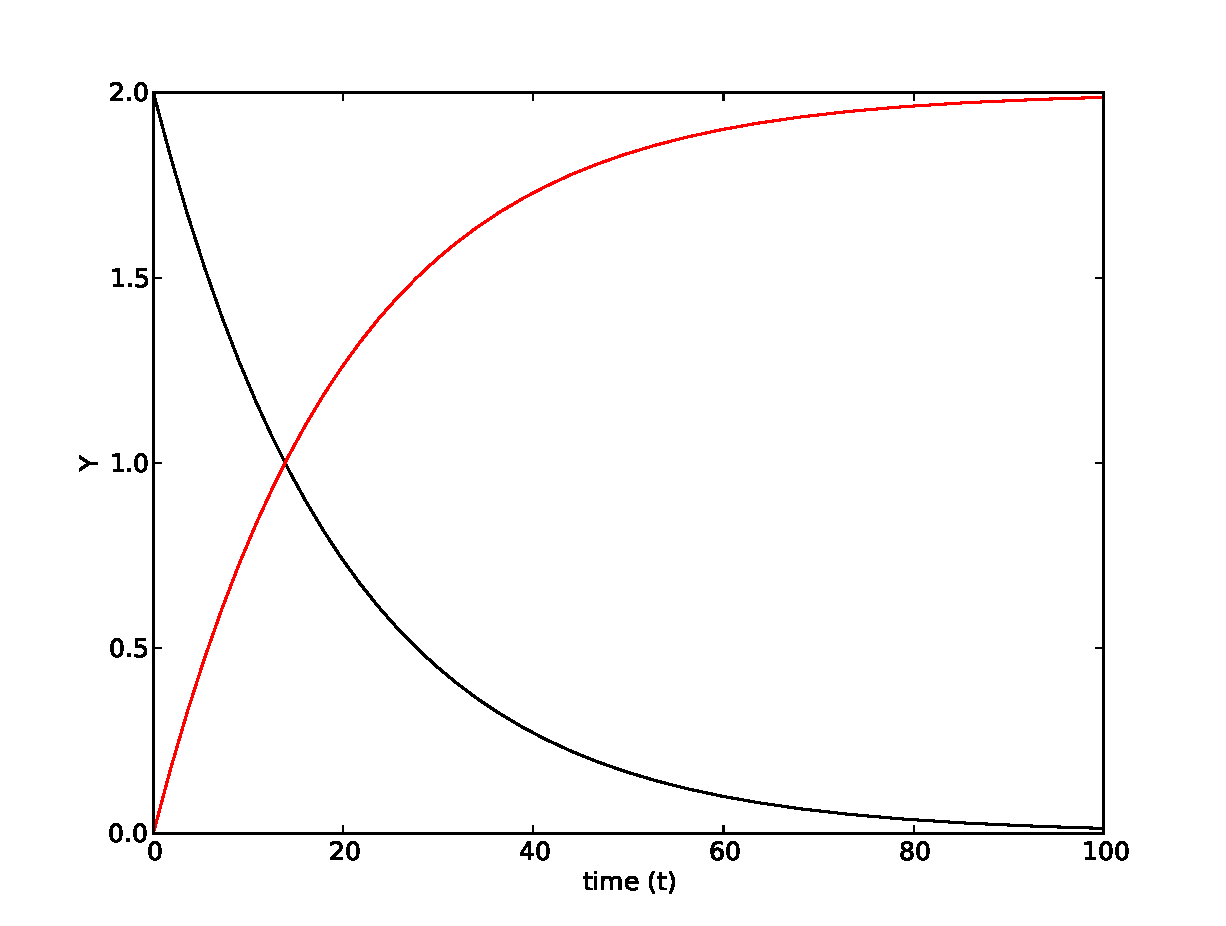
\includegraphics[width=3in]{yst_decayred_accumulateblack_alpha05.pdf}
 \caption{Decay from steady state (black) or accumulation (red) of a protein Y under the logic approximation described above.}
\label{fig:decayaccumulate}
\end{figure}


\subsection{Response Time}

The response time of a system is defined as the time to reach halfway between the initial and final levels in a dynamic process. We'll designate this $T_{1/2}$. If we solve one of the above equations (decay from steady state or build up from zero) by setting $Y(t) = Y_{st}/2$ we fine that following formula for response time:
\[
T_{1/2} = \frac{\log(2)}{\alpha}
\]
%
Interestingly \emph{the response time is only a function of the degradation/dilution rate}, not the rate of production!  This leads us to an important rule of thumb for signaling and regulatory network -- proteins with key roles in signal transduction (as well as modifications like phosphorylation) must have high turnover rates if their concentration need to be adjusted quickly.

\section{Feed Forward Loops}

\begin{figure}[lht]
\centering
 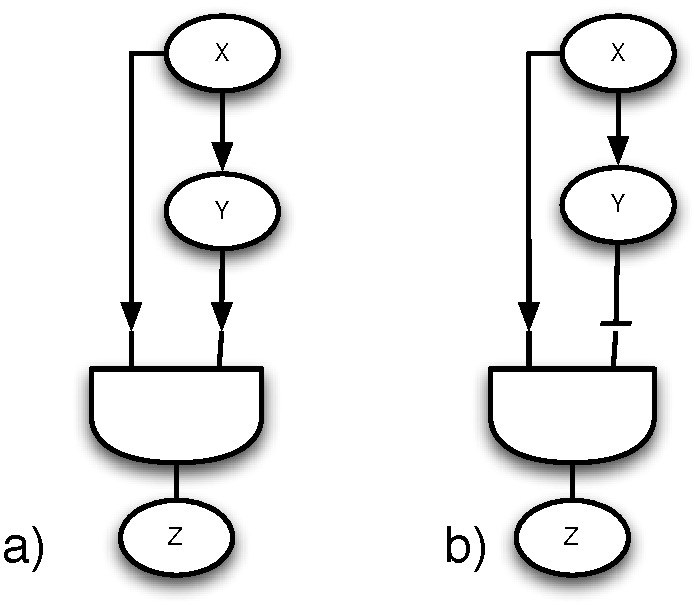
\includegraphics[width=2in]{FFLs.pdf}
\caption{a) A coherent feed forward loop; b) an incoherent feed forward loop.}
\label{fig:FFL}
\end{figure}

We're now going to use some of these tools to look at a class of network motifs, called Feed Forward Loops (FFLs), found in signaling and regulatory networks. FFLs involve interactions between three components, with the basic topology illustrated in \cref{fig:FFL}. Depending on the signs of the edges (whether activating or repressing) we can classify FFLs as `coherent' or `incoherent.' We'll take a look at an example of each class.


\subsection{A Coherent FFL}

The most common type of coherent FFL is illustrated in Fig.~\ref{fig:FFL}a.  In this system X is an activator of Y and both X and Y regulate the production of Z with AND logic (i.e. both X and Y must be above particular thresholds in order to trigger the production of Z). Using our logic approximation framework we will model this network as follows.
\begin{itemize}
    \item For Y:
\begin{eqnarray*}
Y = f(X) = \beta_y\ \Theta(X > K_{xy})
\\
\\
\frac{dY}{dt} = \beta_y\ \Theta(X > K_{xy}) - \alpha_{y}Y
\end{eqnarray*}

    \item For Z:
\begin{eqnarray*}
Z = g(X,Y) = \beta_z\ \Theta(X > K_{xz})\Theta(Y > K_{yz})
\\
\\
\frac{dZ}{dt} = \beta_z\ \Theta(X > K_{xz})\Theta(Y > K_{yz}) - \alpha_{z}Z
\end{eqnarray*}

\end{itemize}

As before we can solve for Y as a function of time and calculate what it's steady state value will be:

\[
Y(t) = Y_{st}(1-e^{-\alpha_{y}t})
\]
and
\[
Y_{st}=\beta_y/\alpha_y
\]

\begin{figure}[lht]
\centering
 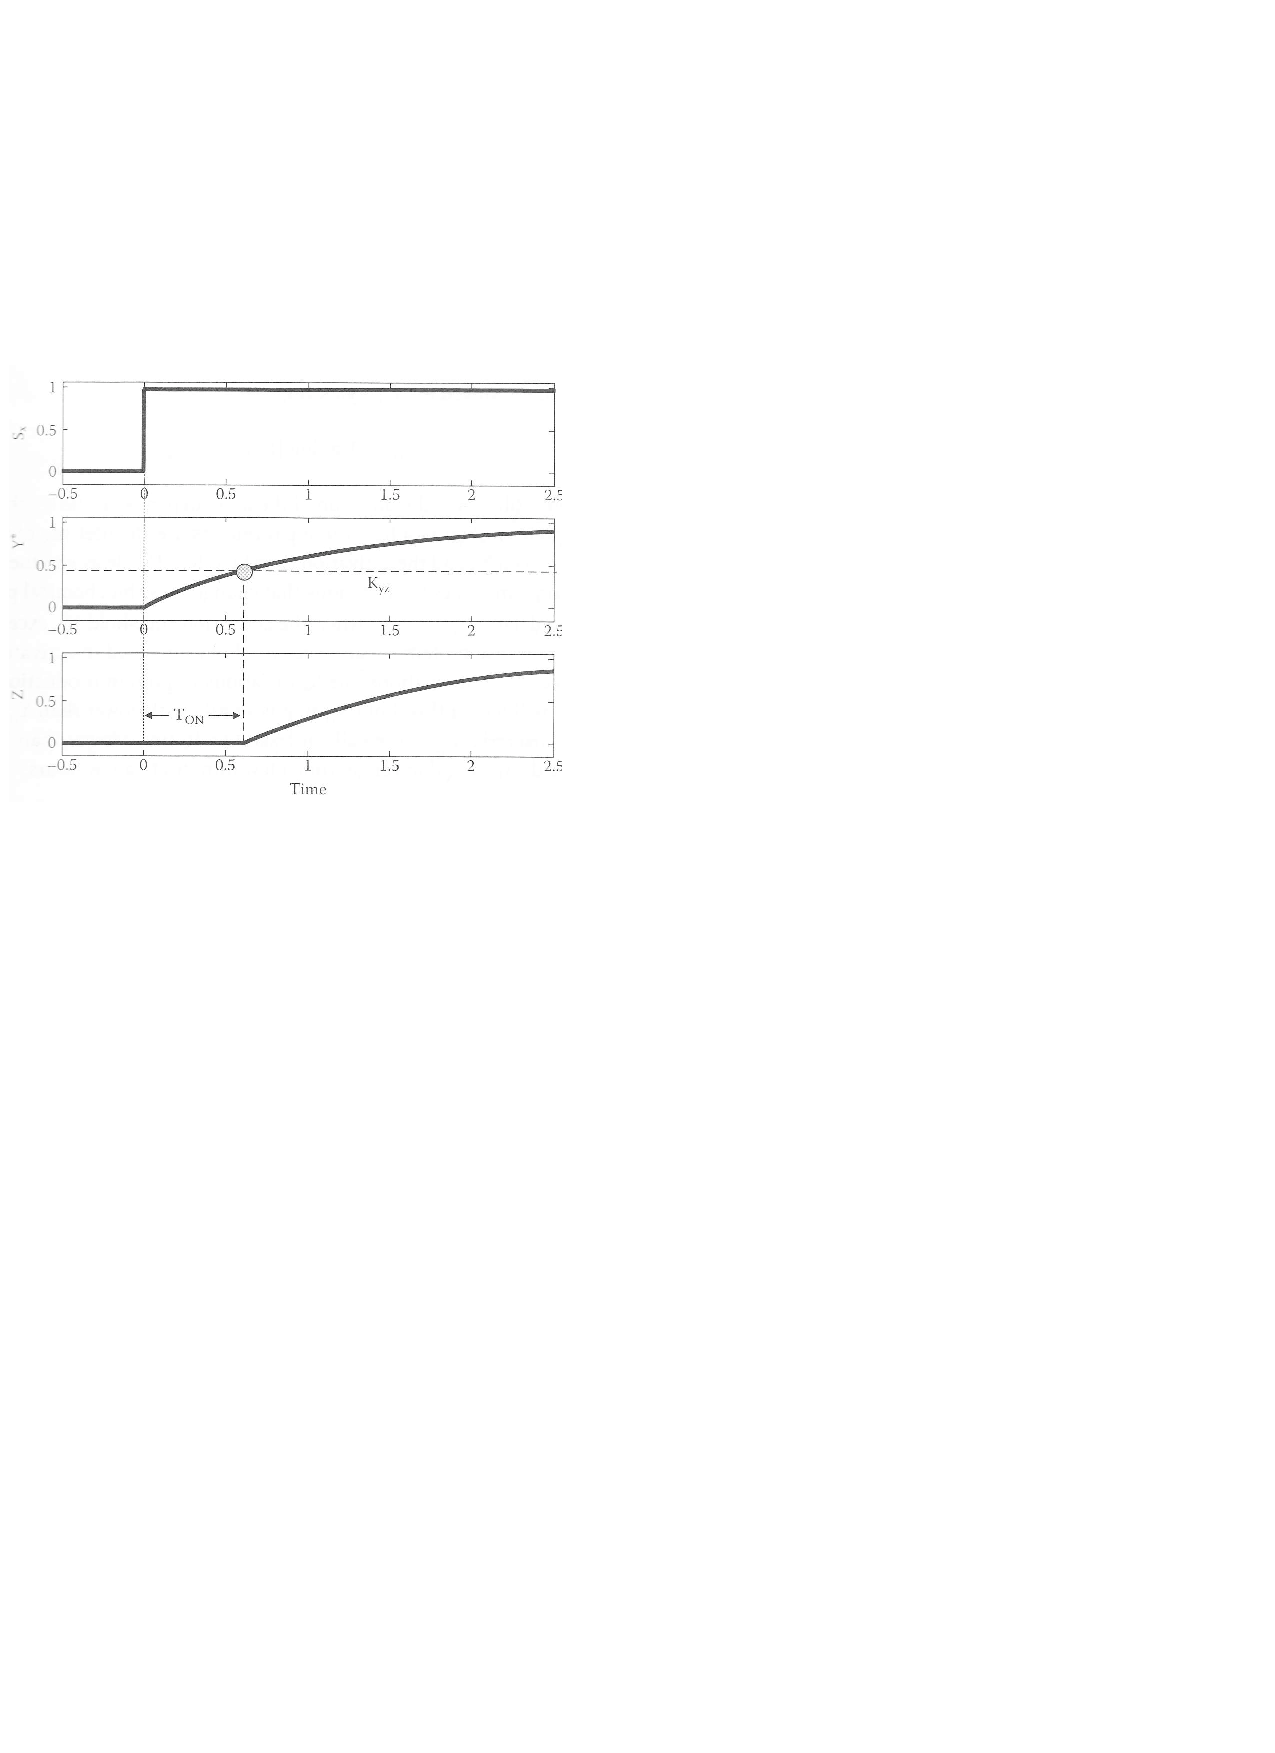
\includegraphics[width=3in]{coh-ffl-Ton.pdf}
\caption{Delay time, $T_{\mathrm{on}}$, associated with a coherent FFL, figure from \cite{Alon2007book}.}
\label{fig:fflton}
\end{figure}


How about Z? Since Z is governed by an AND function it needs both X and Y to be above their respective thresholds, $K_{xz}$ and $K_{yz}$. For the sake of simplicity let's assume that both Y and Z have the same threshold with respect to X, i.e. $K_{xy} = K_{xz}$. This allows us just to consider how long it takes for Y to reach the threshold value $K_{yz}$. Given this we can calculate the delay before Z turns on, $T_{\mathrm{on}}$ as follows.
%
\[
Y(T_{\mathrm{on}}) = Y_{st}(1-e^{-\alpha_y T_{\mathrm{on}}}) = K_{yz}
\]
and solving for $T_{\mathrm{on}}$ we find:
\[
T_{\mathrm{on}} = 1/\alpha_y \log[1/(1-K_{yz}/Y_{st})]
\]
%
Thus we see that the delay before Z turns on is a function of the degradation rate of Y and the ratio between $Y_{st}$ and $K_{yz}$.  This delay in the production on Z is illustrated in Fig.~\ref{fig:fflton}.


As discussed in the article by Shen-Orr et al. \cite{Shen-Orr2002} a feed forward loop of the type we've just discussed can act as a type of filter -- a sign-sensitive delay that keeps Z from firing in response to transient noisy signals from X, but shuts down Z immediately once the signal from X is removed. In Fig.~\ref{fig:fflcoh} we illustrate the dynamics of Y and Z to a short and long input signal X.

\begin{figure}[lht]
\centering
 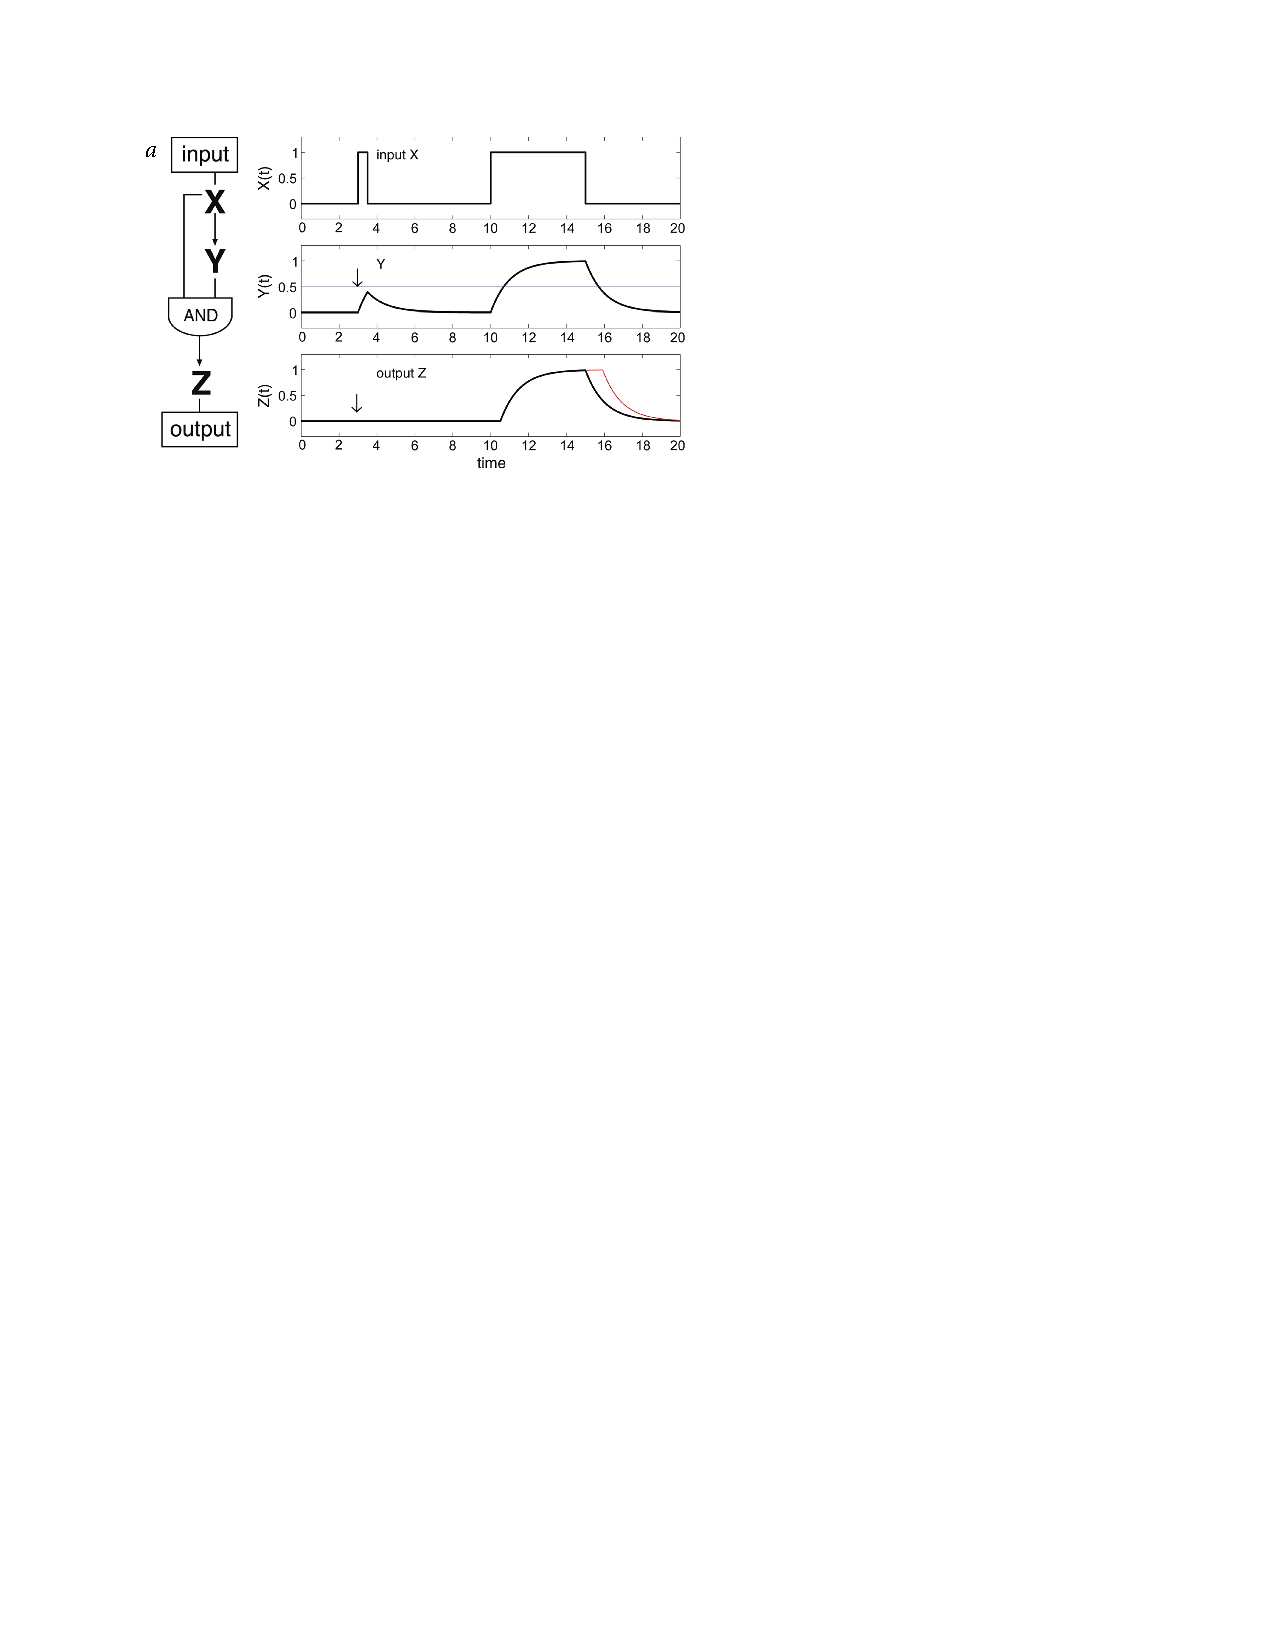
\includegraphics[width=3.5in]{ffl-coherent.pdf}
\caption{Dynamics of a coherent FFL, figure from \cite{Shen-Orr2002}.}
\label{fig:fflcoh}
\end{figure}

\subsection{An Incoherent FFL}

Consider the FFL illustrated in Fig.~\ref{fig:FFL}b.  In this incoherent FFL, the logic function that regulates Z is `X and NOT Y'. That is Z turns on once X is above a given threshold, but only stays on fully as long as Y is below another threshold. Again for simplicity we assume $K_{xy} = K_{yz}$. As before, the dynamics of Y are described by:
\[
\frac{dY}{dt} = \beta_y\ \Theta(X > K_{xy}) - \alpha_{y}Y
\]
and
\[
Y(t) = Y_{st}(1-e^{-\alpha_{y}t})
\]
%
To describe Z we consider two phases - 1) while $Y < K_{yz}$ and 2) while $Y > K_{yz}$. For the first phase:
%
\[
\frac{dZ}{dt} = \beta_z\ \Theta(X > K_{xz}) - \alpha_{z}Z
\]
and
\[
Z(t) = Z_{m}(1-e^{-\alpha_{z}t})
\]

\begin{figure}[lht]
\centering
 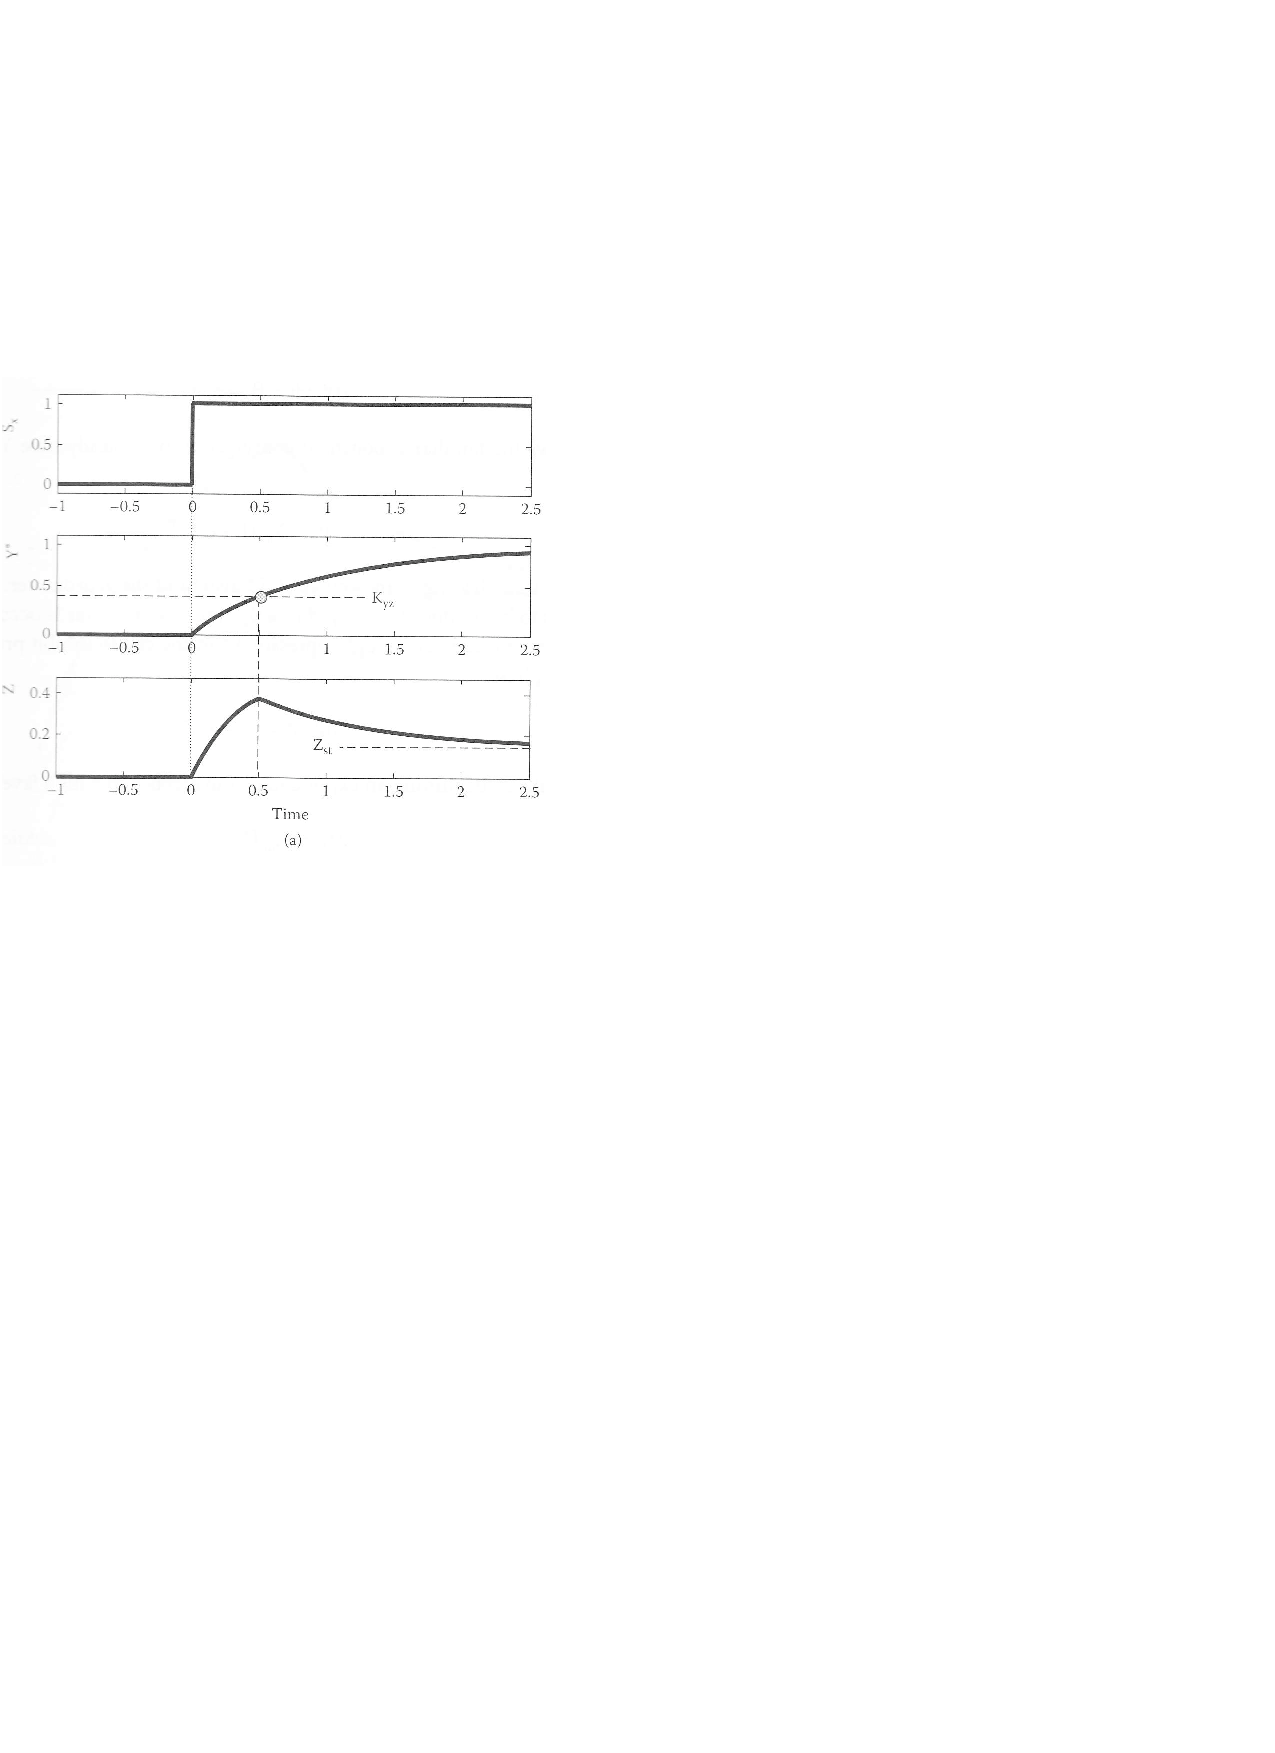
\includegraphics[width=3in]{incoh-ffl-trep.pdf}
\caption{The dynamics of an incoherent FFL illustrated in Fig.~\ref{fig:FFL}b. Figure from \cite{Alon2007}.}
\label{fig:incohffltrep}
\end{figure}


As we did in the case of the coherent FFL, we can calculate the time until Y reaches the treshold $K_{yz}$. We'll call this $T_{\mathrm{rep}}$ and it is the same formula we found for $T_{\mathrm{on}}$ previously.
%
\[
T_{\mathrm{rep}} = \frac{1}{\alpha_y \log[\frac{1}{1-K_{yz}/Y_{st}}]}
\]
%
After a delay, $T_{\mathrm{rep}}$, Y starts to repress the transcription of Z and Z decays to a new lower steady state, $Z_{st} = \beta_{z}^{'}$. The value of  $\beta_{z}^{'}$ depends on how leaky the repression of Z is by Y.  The dynamics of Z in Phase 2 is given by:
%
\[
Z(t) = Z_{st} + (Z_0 - Z_{st})e^{-\alpha_{z}(t-T_{\mathrm{rep}})}
\]
where
\[
Z_0 = Z_{m}(1-e^{-\alpha_{z}T_{\mathrm{rep}}})
\]

The dynamics of X, Y, and Z for a FFL of this type are illustrated in \cref{fig:incohffltrep}.  Note that the stimulus amount of Z in the system initially increases, but then decreases to a lower steady even though the initial stimulus persists. This system thus generates pulse-like dynamics to a persistent signal. How pulse-like the signal is depends on the ratio of $\beta_z$ to $\beta_{z}^{'}$. We define the repression factor, $F$, as follows:
%
\[
F = \frac{\beta_z}{\beta_{z}^{'}} = \frac{Z_m}{Z_{st}}
\]
%
\cref{fig:incohfflpulse} illustrates how varying the repression factor $F$ affects the dynamics of Z.

\begin{figure}[lht]
\centering
 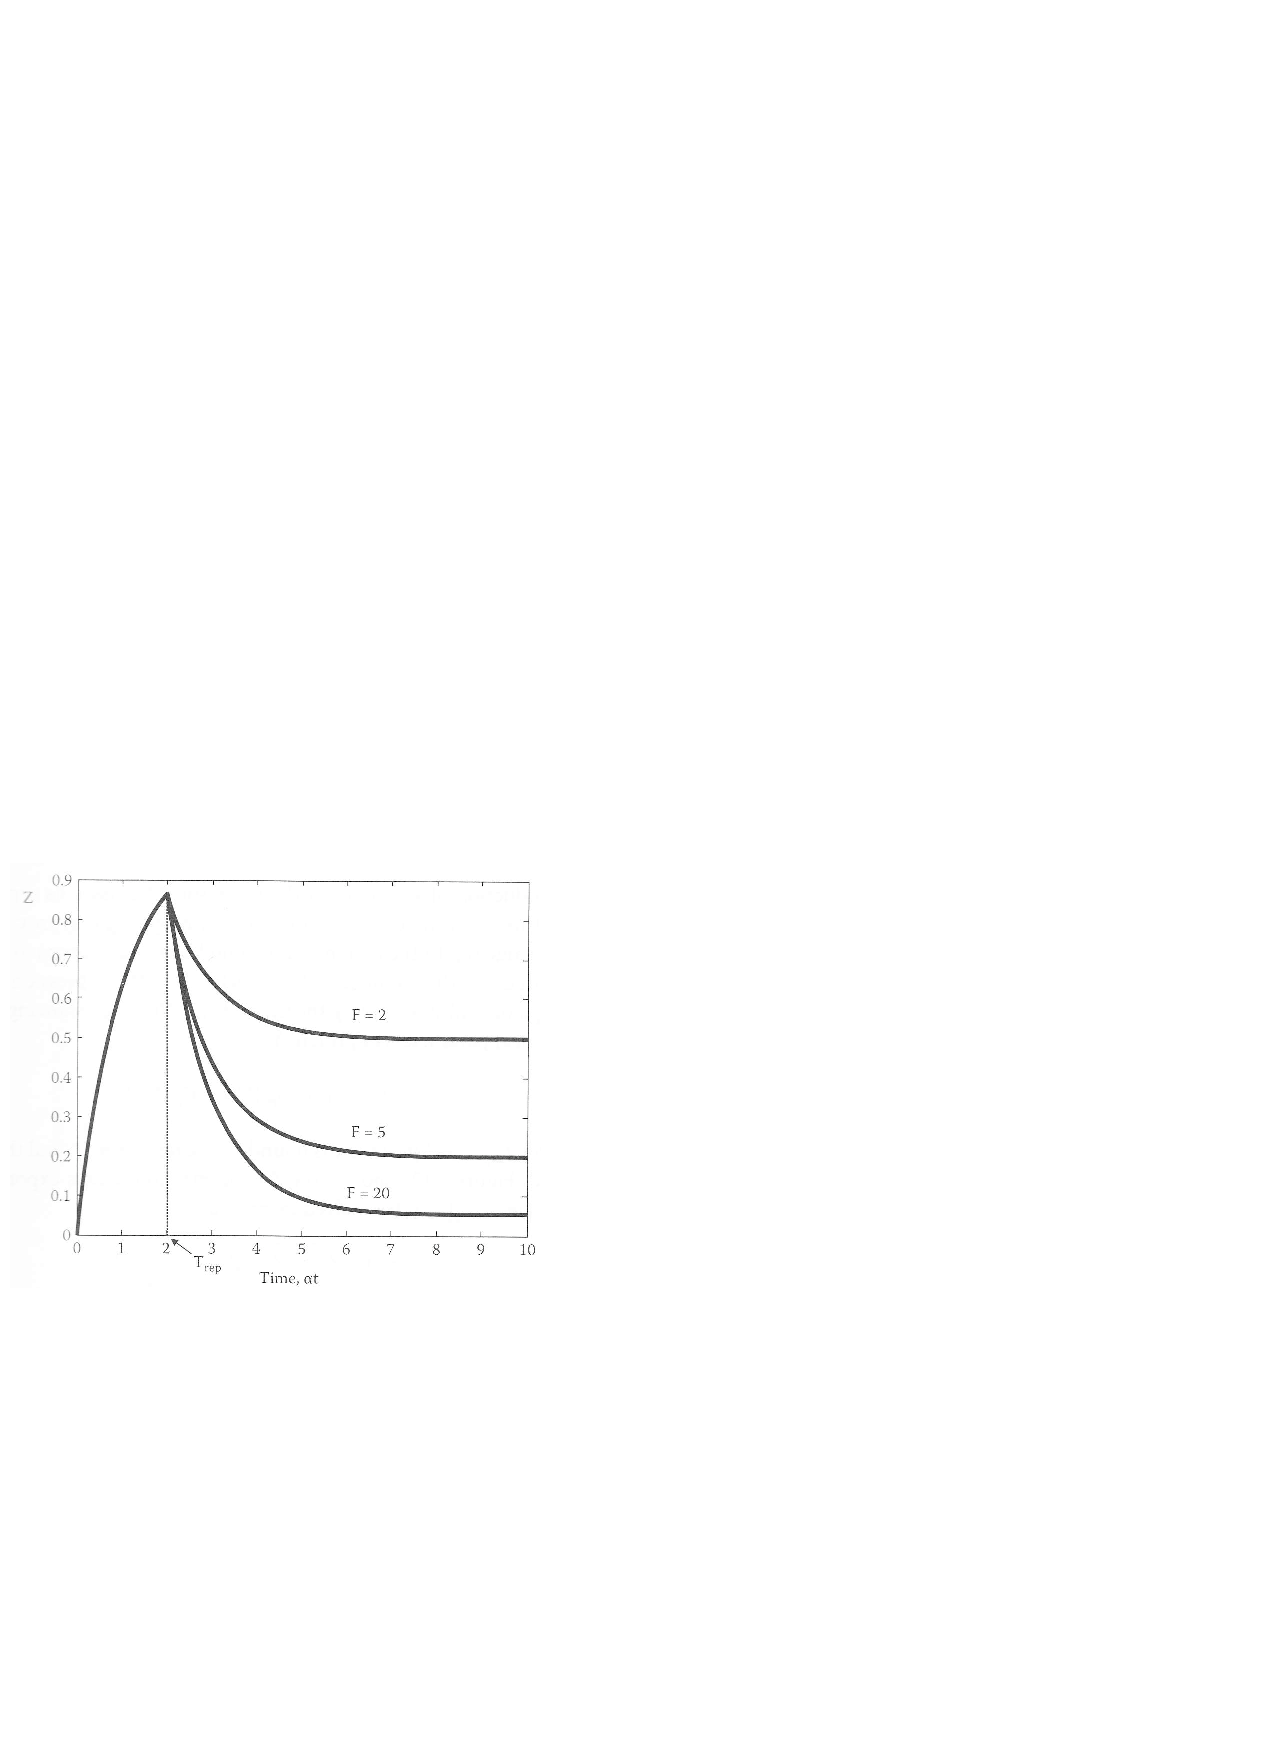
\includegraphics[width=3in]{incoh-ffl-pulse.pdf}
\caption{The effect of varying the repression factor, $F$, on the dynamics of an incoherent FFL. Figure from \cite{Alon2007book}.}
\label{fig:incohfflpulse}
\end{figure}

\subsection{Multiple FFLs}

Multiple FFLs can be link together to generate very complicated dynamics, such as cascades of gene activity such as those often observed in development.  One example, involving both coherent and incoherent FFLs is illustrated in Fig.~\ref{fig:multiffl}.

\begin{figure}[lht]
\centering
 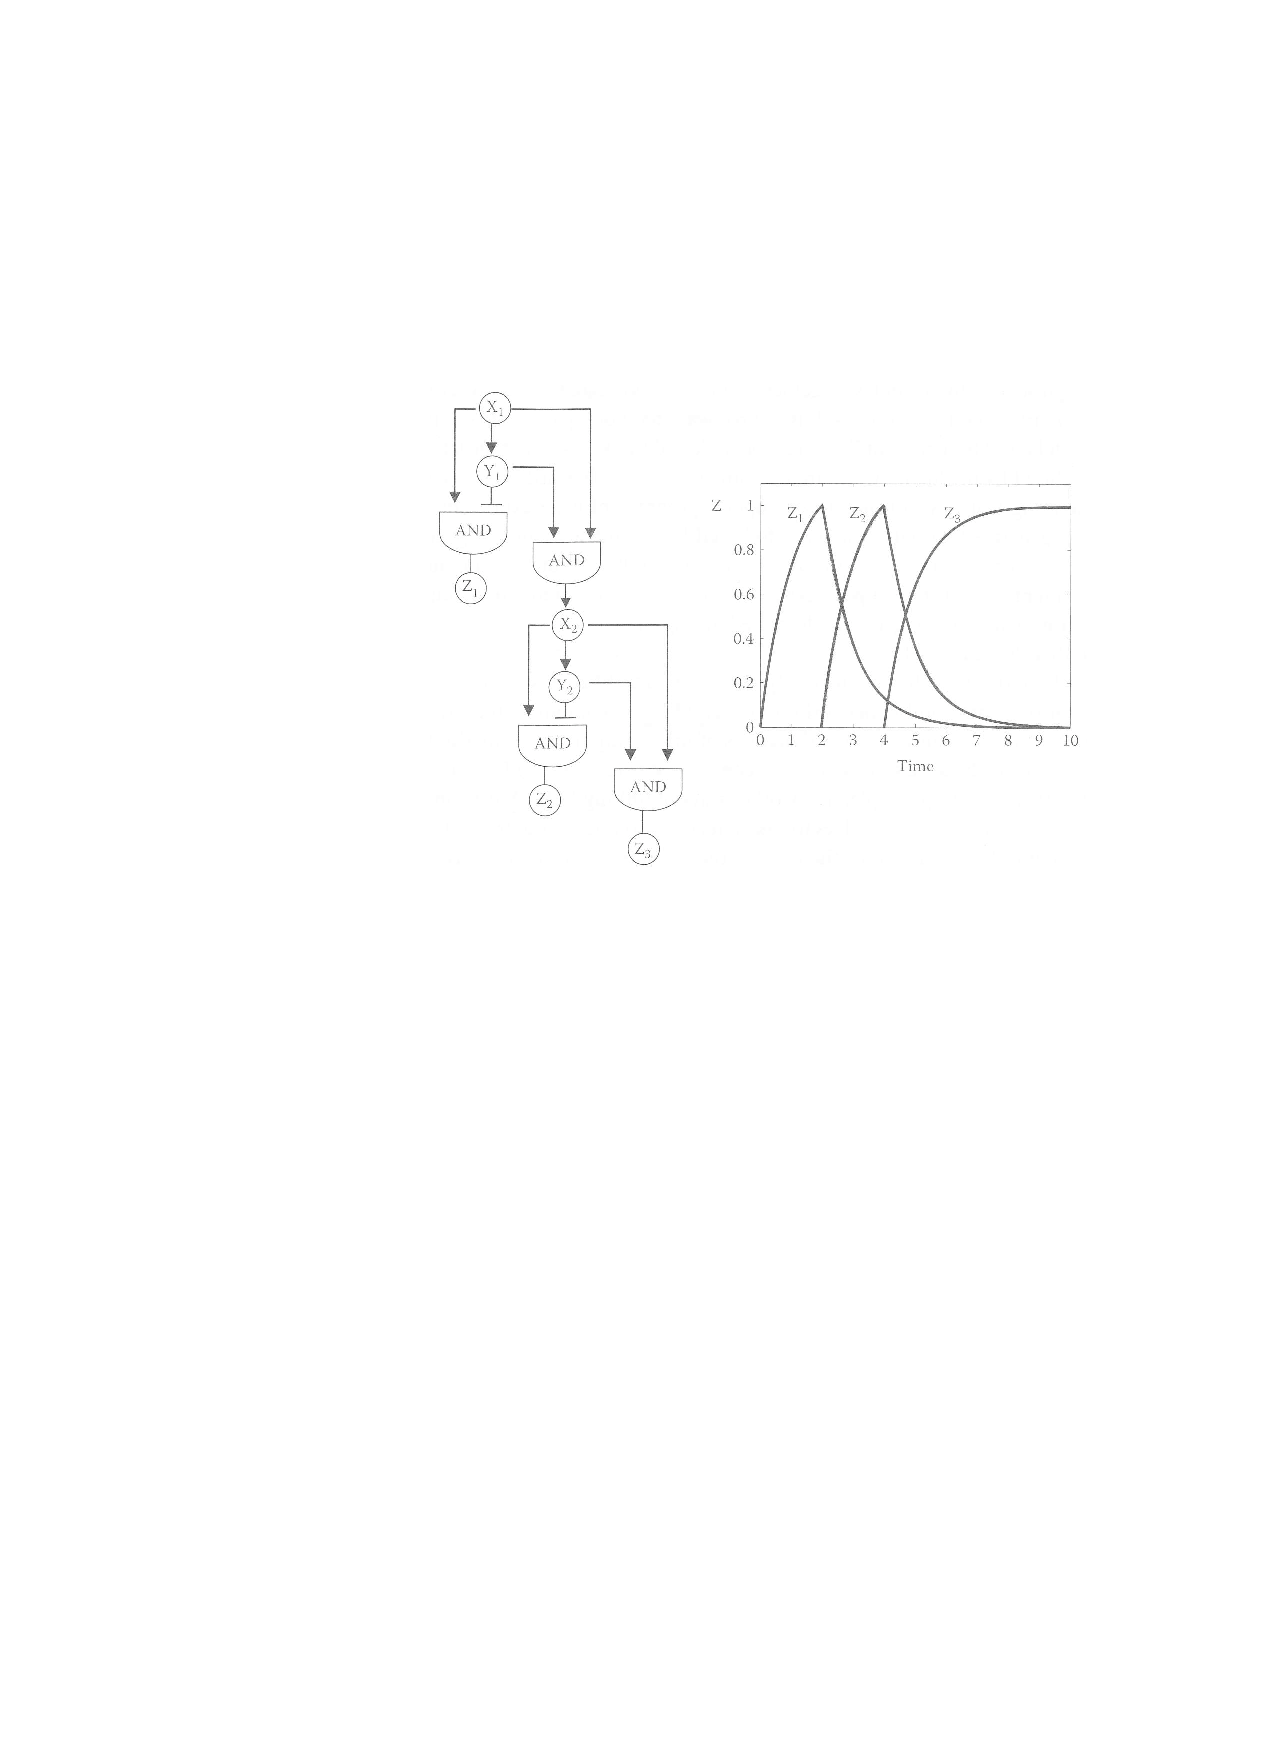
\includegraphics[width=4in]{multiffl.pdf}
\caption{A complex network involving multiple FFLs, both coherent and incoherent, chained together. Figure from \cite{Alon2007book}.}
\label{fig:multiffl}
\end{figure}

\end{document}